\chapter[Visualización]{Estudio de los datos.}
Para poder elegir una estrategia para el preprocesamiento es necesario realizar una visualización de los datos. De esta forma, podremos obtener cómo están distribuidos los valores de cada uno de los atributos o si existe alguna relación de correlación entre ellos.En primer lugar, veamos las distribución de las variables categóricas $ip$, $app$, $channel$, $device$ y $os$.
\begin{figure}[H]
	\centering
	\begin{subfigure}{.5\textwidth}
		\centering
		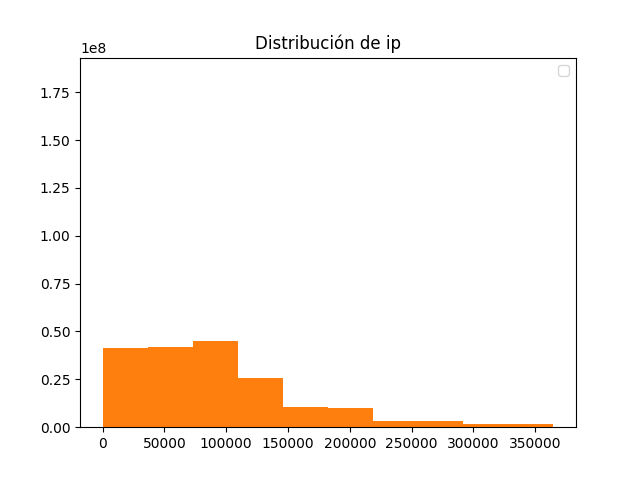
\includegraphics[scale=0.5]{img/ip_distribution.png}
	\end{subfigure}%
	\begin{subfigure}{.5\textwidth}
		\centering
		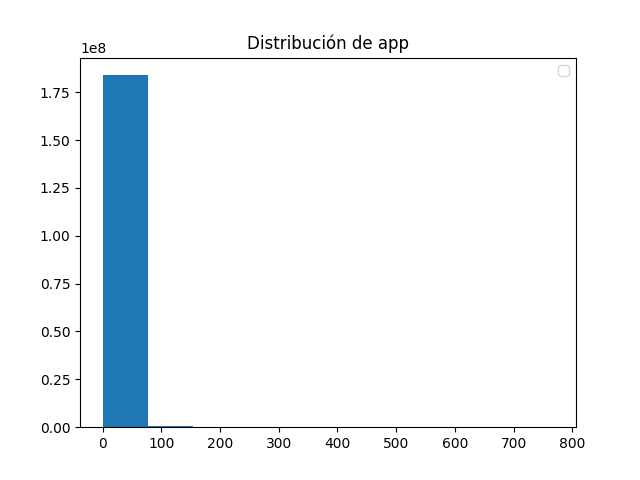
\includegraphics[scale=0.5]{img/app_distribution.png}
	\end{subfigure}
	\caption{Distribución de $ip$ y $app$}
\end{figure}
\begin{figure}[H]
	\centering
	\begin{subfigure}{.5\textwidth}
		\centering
		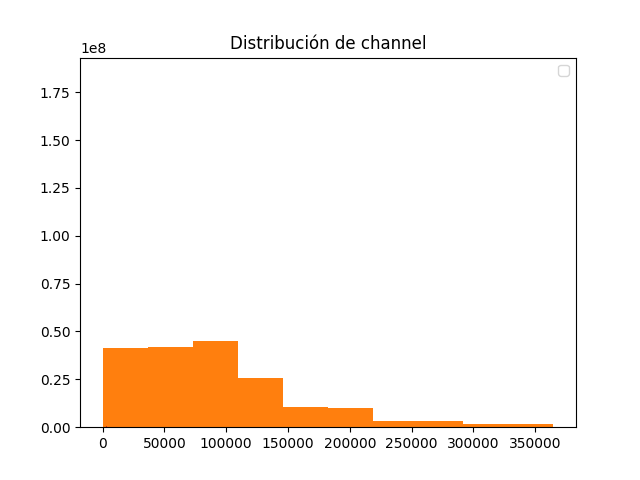
\includegraphics[scale=0.5]{img/channel_distribution.png}
	\end{subfigure}%
	\begin{subfigure}{.5\textwidth}
		\centering
		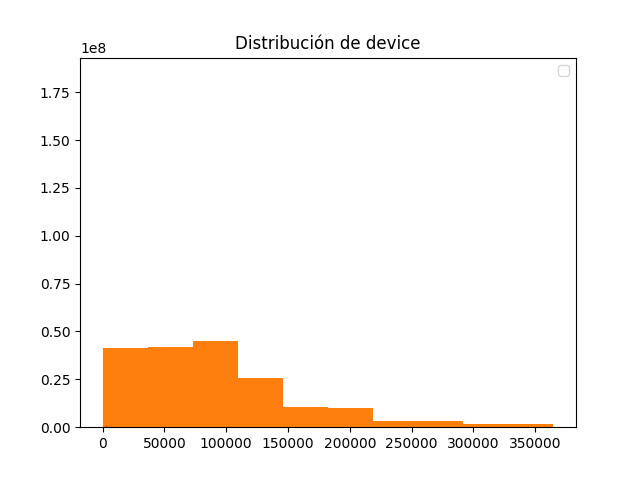
\includegraphics[scale=0.5]{img/device_distribution.png}
	\end{subfigure}
	\caption{Distribución de $channel$ y $device$}
\end{figure}

	\begin{figure}[H]
	\centering
	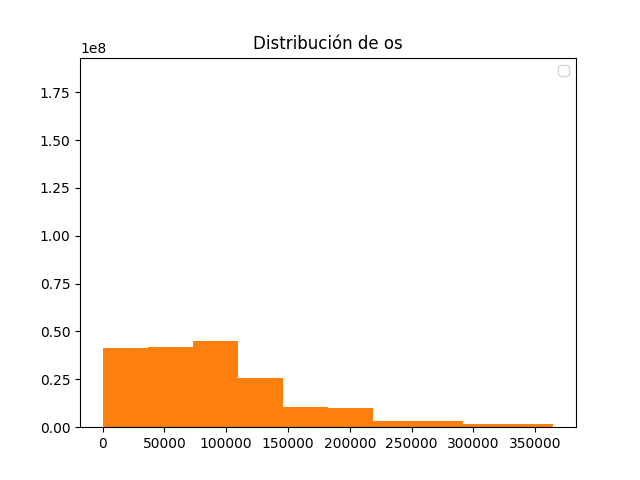
\includegraphics[scale=0.5]{img/os_distribution.png}
	\caption{Distribución de os}
	\end{figure}
Podemos observar que aunque los valores no se concentran en torno a un valor, la distribución no es uniforme.
\medskip

Ahora, estudiaremos la variable $click\_time$. Al tratarse de una variable que representa una hora y fecha, la dividiremos en día, mes, año y valor timestamp(segundos transcurridos desde una fecha fijada por el sistema operativo).
\begin{figure}[H]
	\centering
	\begin{subfigure}{.5\textwidth}
		\centering
		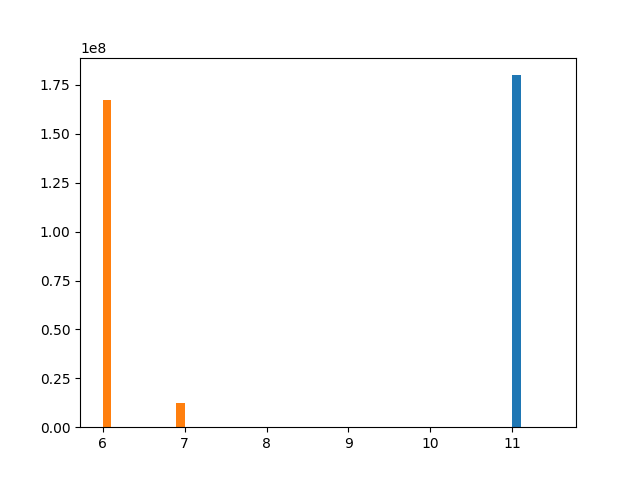
\includegraphics[scale=0.45]{img/click_time_day_distribution.png}
	\end{subfigure}%
	\begin{subfigure}{.5\textwidth}
		\centering
		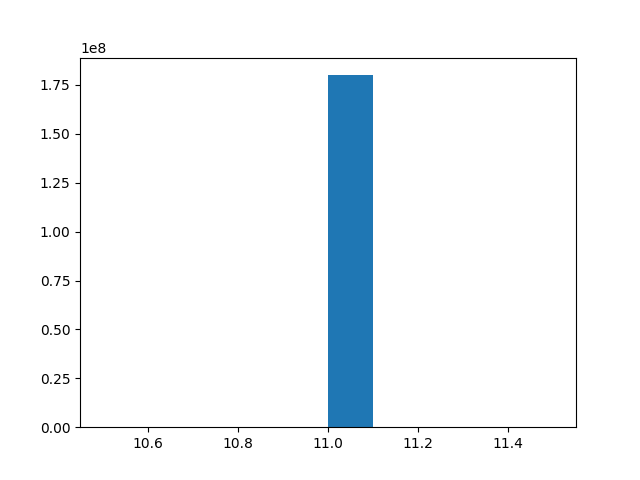
\includegraphics[scale=0.45]{img/click_time_month_distribution.png}
	\end{subfigure}
	\caption{Distribución de $day$ y $month$}
\end{figure}
\begin{figure}[H]
	\centering
	\begin{subfigure}{.5\textwidth}
		\centering
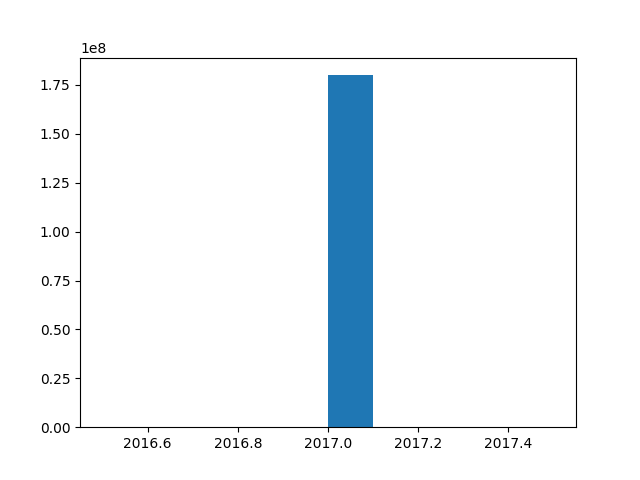
\includegraphics[scale=0.5]{img/click_time_year_distribution.png}
	\end{subfigure}%
	\begin{subfigure}{.5\textwidth}
		\centering
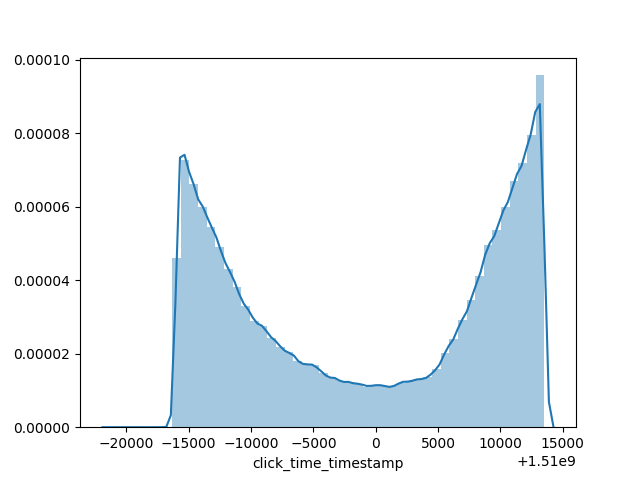
\includegraphics[scale=0.5]{img/normalDistclick_time_timestamp.png}
		
	\end{subfigure}
	\caption{Distribución de $year$ y $timestamp$}

\end{figure}

En esta ocasión sí podemos establecer valores fijos para algunos campos:
\begin{itemize}
	\item Los datos corresponden a los días 6,7 y 8.
	\item Todos los valores corresponden al mes 11.
	\item Todos los registros son del año 2017.
\end{itemize}

Finalmente, estudiaremos el balanceo de clases de la variable a clasificar. Cabe recordar que los clasificadores estándar tienden a sobreaprender la clase mayoritaria, ignorando la minoritaria. En el siguiente gráfico podemos observar que el desbalanceo de clases es más que evidente. Por tanto, los algoritmos a desarrollar deberán tener en cuenta esta característica del conjunto de datos.
\begin{figure}[H]
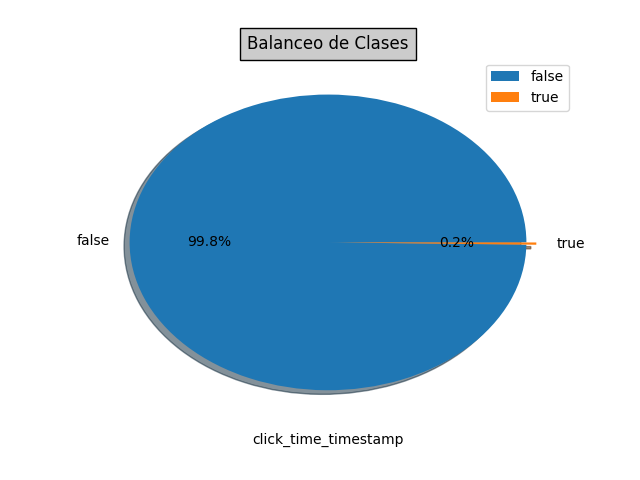
\includegraphics[scale=0.65]{img/imbalacing.png}
\label{}
\caption{Balanceo de clases}
\end{figure}

Una vez hemos visto cómo se distribuyen los datos, a continuación calcularemos el número de valores desconocidos de cada columna. Esta información nos será de ayuda para detectar si una variable no aporta información. Los resultados obtenidos se muestran en la siguiente tabla.
\begin{table}[H]
	\centering
	\begin{tabular}{lllll}
	Atributo& Total & \%    \\
	ip	& 0 &0 \\
	app	& 0 & 0   \\
	os	& 0 & 0 \\
	chanel &0 & 0 \\
	device & 0 & 0  \\
	click\_time& 0& 0 \\
	attributed\_time &184447044& 99.7529
	\end{tabular}
	\caption{Valores perdidos.}
\label{}
\end{table}
A la vista de los resultados obtenidos, podemos afirmar que la variable attributed\_time no nos aporta información debido a que el número de instancias para las que existen valores, es ínfimo. En consecuencia, una de las decisiones a tomar durante la fase de preprocesamiento será no tener en cuenta estos datos en nuestro conjunto de entrenamiento.
\medskip

Finalmente, obtenemos la matriz de correlación entre las variables categóricas usando el coeficiente de correlación de Spearman. 
\begin{figure}[H]
	\centering
	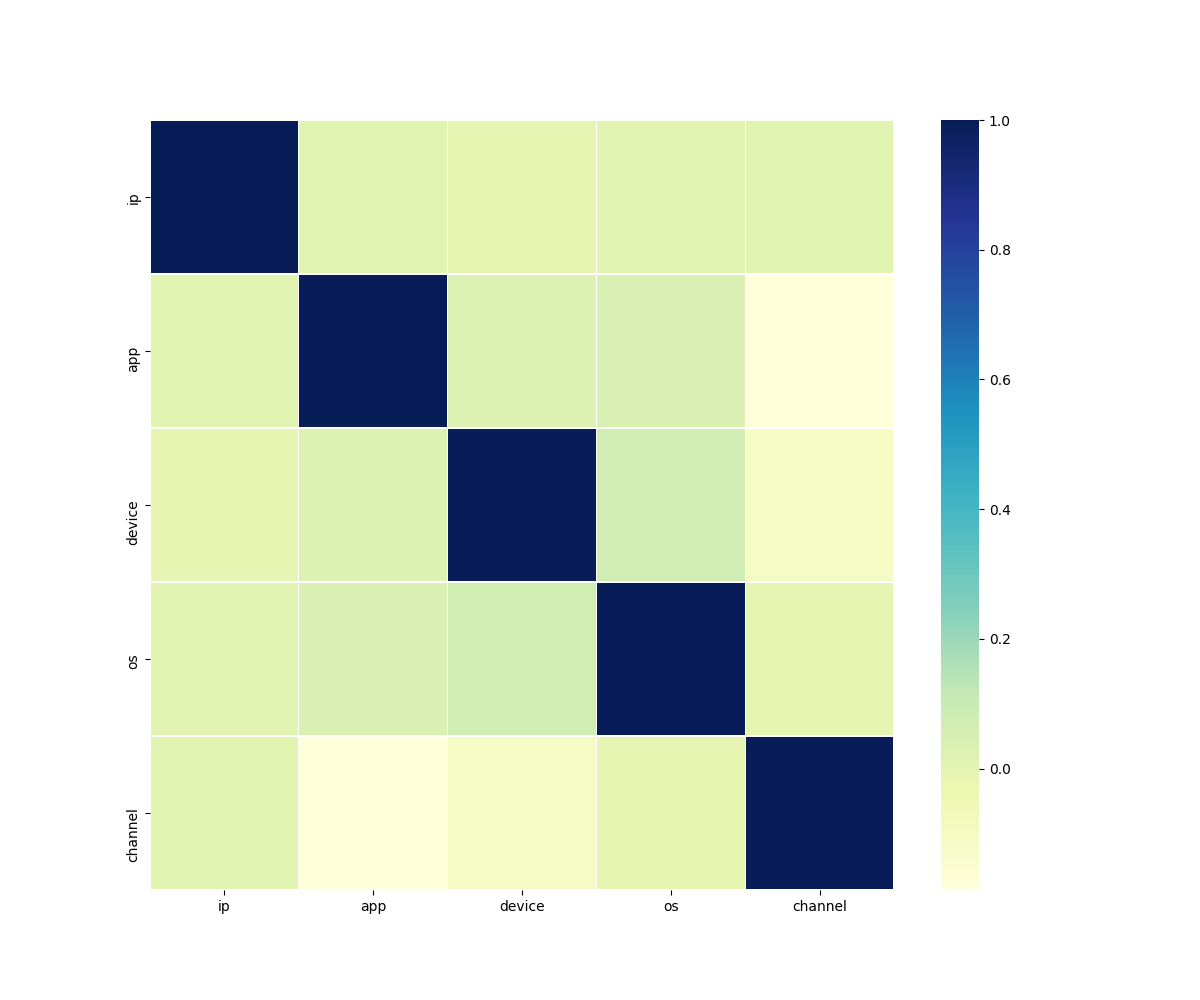
\includegraphics[scale=0.5]{img/correlation.png}
	\caption{Matriz de correlación.}
\end{figure}
Observando el gráfico y teniendo en cuenta que el grado de correlación varía desde 0 hasta 1. Para este estudio, sólo vamos a tener en cuenta aquellas variables con una relación fuerte(valores cercanos a 1). Por tanto, podemos concluir que las variables device y os están relacionadas, mientras que no existen relación entre las demás variables.